%1. Grundlagen
\chapter{Grundlagen}
Diese Studienarbeit befasst sich mit dem komplexen Thema der Elliptischen Kurven in der Kryptographie. Die Kryptographie ist ein mathematisches Thema, bei welchem es zu Anfang der Legung einer Grundlage für das Verständnis der Inhalte dieser Studienarbeit bedarf. In diesem Kapitel werden sowohl die mathematischen als auch die kryptographischen Grundlagen zum Verständnis der Inhalte dieser Studienarbeit gelegt.


\section{Primzahlen}
In der Zahlentheorie, einem Teilbereich der Mathematik, werden viele unterschiedliche Eigenschaften von Zahlen untersucht. Durch die Untersuchung erhofft man sich neue Erkenntnisse für Wissenschaft und Technik. Die Primzahlen als mathematisches Forschungsgebiet sind hierbei ein Teilbereich der Zahlentheorie. Im Folgenden werden Primzahlen definiert und deren Eigenschaften erläutert. Anschließend wird untersucht, wie Primzahlen berechnet werden können. Am Ende wird erläutert, welche Rolle Primzahlen in der Kryptologie und modernen Kryptosystemen innehaben.

\subsection{Definition und Eigenschaften}
Es gibt viele unterschiedliche Zahlenmengen. Beispielsweise gibt es die Menge der reellen Zahlen $\mathbb{R}$. Diese beinhalten als Teilmenge die rationalen und die irrationalen Zahlen. Die natürlichen Zahlen $\mathbb{N}$ bilden hierbei alle positiven ganzen Zahlen ab. Dabei gibt es $\mathbb{N^{+}}$ exklusive der Zahl 0 als Teilmenge mit \[\mathbb{N^{+}} = \{1, 2, 3, 4, 5, ...\}\] und $\mathbb{N}_0$ inklusive der Zahl 0 als Teilmenge mit \[\mathbb{N}_0 = \{0, 1, 2, 3, 4, 5, ...\}.\] Die Primzahlen $\mathbb{P}$ sind hierbei etwas ganz besonderes. Sie unterscheiden sich von anderen Zahlen. Sie sind eine Teilmenge der natürlichen Zahlen und die Kardinalität ihrer Elemente ist unendlich respektive die Anzahl der Primzahlen ist unendlich. Die Unendlichkeit der Primzahlen konnte schon mit mehreren mathematischen Sätzen bewiesen werden, unter anderem dem Satz von Euklid. Auf die unendlichkeit der Primzahlen sowie deren bestimmung wird später in \ref{sec:bestimmung_primzahlen} eingegangen.\\

Doch wie genau sind Primzahlen definiert? Dafür muss erst geklärt werden, was zusammengesetzte Zahlen sind. Dadurch können die Primzahlen klarer von anderen natürlichen Zahlen abgegrenzt werden. Eine natürliche Zahl mit n $\geq$ 2 ist eine zusammengesetzte Zahl, falls es zwei natürliche Zahlen m und k mit den Eigenschaften:

\begin{center}
 m, k $\geq$ 2 oder m, k $\neq$ n, für die gilt: m $\cdot$ k = n. 
\end{center}
 
Zusammengesetzte natürliche Zahlen können also immer als Produkt zweier natürlicher Zahlen $\geq$ 2 beschrieben werden. Primzahlen bilden hierzu das Gegenstück. Eine Primzahl p ist eine natürliche Zahl mit p $\geq$ 1, wobei p nur durch 1 und sich selbst teilbar sein darf. Durch diese Eigenschaft sind Primzahlen nicht zusammengesetzt. Sie können weder als Produkt von natürlichen Zahlen n mit n $\geq$ 2 noch als Produkt von zwei Primzahlen beschrieben werden. Man nehme als Beispiel die Primzahl 7. Sie lässt sich nicht als Produkt von natürlichen Zahlen oder als Produkt von Primzahlen darstellen. Als Gegenbeispiel nimmt man die zusammengesetzte natürliche Zahl 28. Sie kann durch Multiplikation aus den Zahlen 2 und 14 gebildet werden: \[2 \cdot 14=28.\]

Eine weitere Eigenschaft von Primzahlen ist, dass sie das Grundgerüst zur Bildung von Zahlen sind, da man aus ihnen alle natürlichen Zahlen bilden kann. Eine zusammengesetzte natürliche Zahl n mit n $\geq$ 2 kann wie bereits beschrieben immer als Produkt von mindestens zwei weiteren natürlichen Zahlen dargestellt werden. Die einzelnen Faktoren können wiederum ebenfalls als Produkt von zwei weiteren natürlichen Zahlen dargestellt werden. Diese Aufteilung geht rekursiv so lange weiter, bis die Faktoren lediglich Primzahlen sind. Die übrig gebliebenen Faktoren dieses Produktes heißen Primfaktoren. Die Zerlegung einer zusammengesetzten natürlichen Zahl in ihre Primfaktoren nennt man Primfaktorzerlegung. Zweck dieser Primfaktorzerlegung ist es Zahl als Produkt von mehreren Primzahlen darzustellen. Nehmen wir als Beispiel die Zahl 28. Im vorigen Absatz stellten wir diese zusammengesetzte natürliche Zahl durch die Multiplikation von 2 und 14 dar. Die Zahl 2 ist eine Primzahl. Die Zahl 14 ist noch nicht in ihre Primzahlfaktoren zerlegt. Sie lässt sich als folgendes Produkt darstellen: \[2 \cdot 7=14.\] Da 7 auch eine Primzahl ist, wurden alle Primfaktoren gefunden. Die Zahl 28 lässt sich in ihrer Primfaktorzerlegung also wie folgt darstellen: \[2 \cdot 2 \cdot 7=28.\] Die Mehrfachheit von Primzahlen lässt sich auch als Potenz schreiben. Somit wird daraus \[2^{2} \cdot 7=28.\] Der Vorteil durch die Potenzen zeigt sich besonders bei großen Zahlen, da diese oft eine große Anzahl an Primfaktoren haben können. Nimmt man als Beispiel die Zahl 5281250000. Diese setzt sich mit ihren Primfaktoren wie folgt zusammen: \[2 \cdot 2 \cdot 2 \cdot 2 \cdot 5 \cdot 5 \cdot 5 \cdot 5 \cdot 5 \cdot 5 \cdot 5 \cdot 5 \cdot 5 \cdot 13 \cdot 13=5281250000.\] Man erkennt rasch, dass sich die Primfaktoren mit der Potenzschreibweise zusammenfassen lassen und man so die Primfaktorzerlegung wie folgt darstellen kann: \[2^{4} \cdot 5^{9} \cdot 13^{2}=5281250000.\] Die Vorteile der Potenzschreibweise liegt hier auf der Hand, da man erheblich Zeit beim Aufschreiben und Platz auf dem Papier spart.

\subsection{Bestimmung von Primzahlen}\label{sec:bestimmung_primzahlen}
Nachdem die grundlegenen Eigenschaften der Primzahlen angeführt wurden, muss auf die Bestimmung von Primzahlen eingegangen werden. Paulo Ribenboim geht in seinem Buch \glqq\textit{Die Welt der Primzahlen: Geheimnisse und Rekorde}\grqq der Frage auf den Grund, ob primzahldefinierende Funktionen existieren. An einer Stelle des Buches geht er auf diese möglichen Funktionen und ihre Eigenschaften ein \cite[vgl.][S. 137]{Ribenboim.2011}. Solch eine Funktion müsse laut ihm eine der folgenden drei Eigenschaften aufweisen, damit man sie zur Bestimmung von Primzahlen nutzen könne:

\begin{itemize}
\item[ (a) ]  $f(n) = p_n$ (die n-te Primzahl) für alle n $\geq$ 1;
\item[ (b) ]  $f(n)$ ist immer prim und wenn n $\neq$ m, dann gilt: $f(n) \neq f(m)$;
\item[ (c) ]  der positive Wertebereich der Funktion ist identisch mit der Menge der Primzahlen
\end{itemize}

Ribenboin erklärt, dass die Bedingung, um (a) zu erfüllen schärfer sei als (b) und als (c). Die bisher erzielten Resultate zur Findung einer Formel zur Bestimmung von Primzahlen seien außerdem eher enttäuschend. Doch wenn die Funktionen zur Bestimmung von Primzahlen bisher enttäuschend waren, wie wurden diese bisher bestimmt?\\

Eine der simpelsten und sicher auch eine der ältesten Methoden ist das \glqq Sieb des Eratosthenes\grqq . Der Übersetzer Kai Brodersen beschreibt in seiner Übersetzung aus dem Jahre 2021 eines Buches aus dem Griechischen von Nikomachos von Gerasa, wie dieser sehr simpel die Funktionsweise des Siebes erläuterte \cite[vgl.][S. 7]{Nikomachos+2021+7+7}. Die Richtigkeit dieses Verfahrens wurde von Nikomachos im frühen 2. Jh. n. Chr. belegt. Bei dem Verfahren schreibt man alle natürlichen Zahlen von 2 bis zu einer gewählten Zahl n in eine Liste. Um die Primzahlen zu erhalten, siebt man jetzt die zusammengesetzten natürlichen Zahlen aus, indem man Vielfache streicht. Man beginnt bei der kleinsten Zahl, der 2. Man schreitet in der Liste fort und streicht alle Vielfachen der 2 bis zur höchsten gewählten Zahl n durch. Anschließend beginnt man mit der nächstgrößeren Zahl, welche nicht durchgestrichen ist respektive ausgesiebt wurde und streicht von dieser ebenfalls alle Vielfachen bis zur höchsten Zahl n durch. Den simplen Algorithmus führt man nun solange fort, bis man keine Vielfachen mehr streichen kann. Die übriggebliebenen Zahlen sind die Reihe der Primzahlen bis n. Die Darstellung in einer Tabelle ist heutzutage geläufig, da dies übersichtlicher ist. In der folgenden Tabelle wurde der Algorithmus des Siebes des Eratosthenes von 2 bis 100 angewandt:\\

\begin{center}
\begin{tabular}{|c|c|c|c|c|c|c|c|c|c|}
\hline 1 & 2 & 3 & $\not{4}$ & 5 &
$\not{6}$ & 7 & $\not{8}$ & $\not{9}$ & $\not{10}$ \\ \hline 11 & $\not{12}$
& 13 & $\not{14}$ & $\not{15}$ & $\not{16}$ & 17 & $\not{18}$ & 19 &
$\not{20}$ \\ \hline $\not{21}$ & $\not{22}$ & 23 & $\not{24}$ & $\not{25}$
& $\not{26}$ & $\not{27}$ & $\not{28}$ & 29 & $\not{30}$ \\ \hline 31 &
$\not{32}$ & $\not{33}$ & $\not{34}$ & $\not{35}$ & $\not{36}$ & 37 &
$\not{38}$ & $\not{39}$ & $\not{40}$ \\ \hline 41 & $\not{42}$ & 43 &
$\not{44}$ & $\not{45}$ & $\not{46}$ & 47 & $\not{48}$ & $\not{49}$ &
$\not{50}$ \\ \hline $\not{51}$ & $\not{52}$ & 53 & $\not{54}$ & $\not{55}$
& $\not{56}$ & $\not{57}$ & $\not{58}$ & 59 & $\not{60}$ \\ \hline 61 &
$\not{62}$ & $\not{63}$ & $\not{64}$ & $\not{65}$ & $\not{66}$ & 67 &
$\not{68}$ & $\not{69}$ & $\not{70}$ \\ \hline 71 & $\not{72}$ & 73 &
$\not{74}$ & $\not{75}$ & $\not{76}$ & $\not{77}$ & $\not{78}$ & 79 &
$\not{80}$ \\ \hline $\not{81}$ & $\not{82}$ & 83 & $\not{84}$ & $\not{85}$
& $\not{86}$ & $\not{87}$ & $\not{88}$ & 89 & $\not{90}$ \\ \hline
$\not{91}$ & $\not{92}$ & $\not{93}$ & $\not{94}$ & $\not{95}$ & $\not{96}$
& 97 & $\not{98}$ & $\not{99}$ & $\not{100}$ \\ \hline
\end{tabular}
\end{center}

Das Sieb des Eratosthenes ist eine Möglichkeit, Primzahlen genau zu bestimmen. Problematisch wird es jedoch bei großen Zahlen. Für jede Zahl müssen je alle anderen Zahlen durchgegangen werden und es muss eine Teilbarkeitsprüfung durchgeführt werden. Umso größer die Zahlen werden, umso rechenaufwendiger wird die Anwendung des Sieb des Eratosthenes, um Primzahlen zu finden. Dieses ist also kein optimaler Ansatz, große Primzahlen zu bestimmen. Neben dem Sieb des Eratosthenes gibt es viele weitere Methoden, Primzahlen zu bestimmen.\\

Die Besprechung aller dieser Verfahren und Algorithmen soll nicht Thema dieser Arbeit sein, jedoch soll noch eine gängige Methode erläutert werden. Über Probabilistische Verfahrne kö

WEITERSCHREIBEN

\subsection{Rolle der Primzahlen in der Kryptografie}
Primzahlen haben einen effektiven Nutzen in der Kryptografie. Bevor man sich fragt, wie Primzahlen in der Kryptografie genutzt werden, sollte man die Kryptografie vorher definieren. Dietmar Wätjen beschreibt diesne Begriff seinem Buch \glqq\textit{Kryptographie: Grundlagen, Algorithmen, Protokolle}\grqq aus dem Jahr 2018 \cite[vgl.][S. 1]{Watjen.2018}. Kryptografie ist die Wissenschaft vom geheimen Schreiben. Kernziel ist es dabei, einen unverschlüsselten Text, genannt Klartext in einen Chiffretext überführt. Dieser Vorgang heißt \textit{chiffrieren}. Der Vorgang, bei welchem der Chiffretext wieder in den Klartext überführt wird, heißt \textit{dechiffrieren}. Für beide Vorgänge werden Schlüssel notwendig. Die Abbildung \ref{fig:verschluesselung} stellt dies übersichtlich dar:

\begin{figure}[!h]
    \centering
    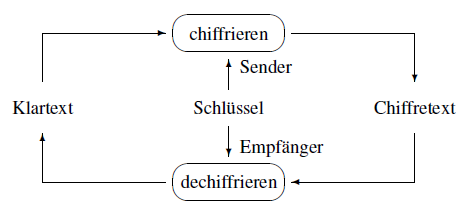
\includegraphics[width=\textwidth]{grafiken/verschluesselung.png}
    \caption[Kryptografische Verschlüsselung]{Kryptografische Verschlüsselung \\ Quelle: \cite{Watjen.2018}}
    \label{fig:verschluesselung}
\end{figure}

Wätjen beshreibt Kryptografische System, auch Kryptosystem genannt, als ein System aus fünf Komponenten:

\begin{itemize}
\item[ 1. ]  Klartextraum $M$
\item[ 2. ]  Chiffretextraum C
\item[ 3. ]  Schlüsselraum K
\item[ 4. ]  Familie von Chiffriertransformationen $E_k:M \rightarrow C$ mit $k \in K$
\item[ 5. ]  Familie von Dehiffriertransformationen $D_k:C \rightarrow M$ mit $k \in K$
\end{itemize}

Laut Watjen sind $M$, $C$ und $K$ höchstens, abzählbare Mengen. Eine Chiffriertransformation $E_K$ wird durch einen Schlüssel $K$ und einen Chiffrieralgorithmus $E$ definiert, welcher für jede Familie gleich ist. Eine Dechiffriertransformation $D_K$ wird ebenfalls durch einen Schhlüssel $K$ bestimmt. Desweiteren sollen die Kryptografischen Systeme nach Watjen die folgenden drei Eigenschaften aufweisen:

\begin{itemize}
\item[ (1) ]  Klartextraum $M$
\item[ (2) ]  Chiffretextraum C
\item[ (3) ]  Schlüsselraum K
\end{itemize}

Laut



Durch die Kryptografie können dadurch Übertragungen von sensiblen Informationen zum einen sicherer als auch privater ablaufen, da ein abgefangenes Chiffrat nicht direkt lesbar ist. 






Primzahlen sind aufgrund ihrer hervorragenden Eigenschaften für die Kryptologie nützlich. Viele Verfahren, welche den Klartext in einen Chiffretext überführen, benötigen für ihren Algorithmus Primzahlen. Ein gutes Beispiel ist der Diffie-Hellmann-Schlüsselaustausch 

hier diffie-hellmann




\section{Algebraische Strukturen}
Definiert durch die Zahlentheorie und als zentraler Untersuchungsgegenstand des mathematischen Teilgebietes der universellen Algebra, liefern algebraische Strukturen die Basis zur Realisierung komplexer symmetrischer und asymmetrischer Kryptosysteme, weshalb wir im folgenden Kapitel die Eigenschaften relevanter algebraischer Strukturen näher betrachten wollen. Darüber hinaus möchten wir Ihnen auch einige Werkzeuge zum Rechnen in der jeweiligen algebraischen Struktur an die Hand geben, welche zur späteren Realisierung von Kryptosystemen benötigt werden.\\

Unter einer sehr allgemeinen Betrachtung ist eine mathematische Struktur eine Liste nichtleerer Mengen, genannt Trägermengen, mit Elementen aus den Trägermengen, genannt Konstanten, und mengentheoretischer Konstruktionen über den Trägermengen. Diese sind konkret Funktionen über den Trägermengen. Im Weiteren beschränken wir uns auf den Fall einer einzigen Trägermenge, wodurch die Strukturen als homogen bezeichnet werden können.

\paragraph{Definition: Homogene algebraische Struktur}
Eine homogene algebraische Struktur ist ein Tupel $(M,c_1,\dots,c_m,f_1,\dots,f_n)$ mit $m,n \in \mathbb{N}$ und $n \geq 1$. Dabei ist $M$ eine nichtleere Menge, genannt \textbf{Trägermenge}, alle $c_i$ sind Elemente aus $M$, genannt die \textbf{Konstanten}, und alle $f_i$ sind $s_i$-stellige Funktionen $f_i:M \rightarrow M$ im Fall $s = 1$ und $f_i:M^{s_i} \rightarrow M$ im Fall $s_i>1$, genannt die (inneren) \textbf{Operationen}. Die lineare Liste$(0,\dots,0,s_1,\dots,s_n)$ mit $m$ Nullen heißt \textbf{Typ} oder die \textbf{Signatur}.\newline

Laut dieser Definition muss eine homogen algebraische Struktur nicht unbedingt Konstanten enthalten, jedoch mindestens eine Operation. Das Paar $(\mathbb{N},+)$ bildet beispielsweise eine homogene algebraische Struktur des Typs (2). Das 5-Tupel $(\mathbb{N},0,1,+,\cdot)$ bildet ebenfalls eine homogen algebraische Struktur des Typs (0,0,2,2).

Algebraische Strukturen unterscheiden sich grundsätzlich durch ihren Typ. Wirklich charakterisiert werden sie aber erst durch die jeweils geltenden Axiome, d.h. bestimmte Eigenschaften, welche für die Konstanten und Operationen gefordert werden. Durch die Hinzunahme immer weiterer Axiome, entsteht eine Hierarchie immer feinerer Strukturen, an deren Anfang der Monoid steht.

\subsection{Monoid}

\paragraph{Definition: Monoid}
Eine algebraische Struktur $(M,e,\cdot)$ des Typs (0,2) heißt ein Monoid, falls für alle $x,y,z\in M$ die folgenden Monoid Axiome gelten:
\begin{itemize}
    \item (Ass) $x \cdot (y \cdot z) = (x \cdot y) \cdot z$
    \item (Neu) $e \cdot x = x = x \cdot e$
\end{itemize}  Gilt zusätzlich noch für alle $x,y \in M$ die Gleichung $x \cdot y = y \cdot x$, so heiß $(M,e,\cdot)$ ein \textbf{kommutatives Monoid}.\\

Die erste und die letzte Gleichung bilden das Assoziativ- und Kommutativgesetz ab. Durch die mittlere Gleichung wird ein neutrales Element $e$ bezüglich der Operation gefordert, wobei sowohl die \textbf{Linksneutralität} als auch die \textbf{Rechtsneutralität} spezifiziert wird.\\

Einfache Beispiele für Monoide sind $(\mathbb{N},0,+)$, $(\mathbb{N},1,\cdot)$ und $(\mathbb{Z},0,+)$. Die Potenzierung in solchen Monoiden ist folgendermaßen definiert.

\paragraph{Definition: Potenzierung}
In einem Monoid $(M,e,\cdot)$ definiert man die $n$-te \textbf{Potenz} $x^n$ von $x \in M$ durch $x^0 := e$ und $x^{x+1} = x \cdot x^n$ für alle $n \in \mathbb{N}$.\\

Daraus ergibt sich für den Monoid $(\mathbb{N},1,\cdot)$ die aus $\mathbb{R}$ gewohnte Potenzierung. Nach welcher für ein $x \in \mathbb{N}$ die Potenzierung $x^n = x_1 \cdot x_2 \cdot \dots \cdot x_n$ ergibt. Betrachtet man jedoch den Monoid $(\mathbb{N},0,+)$, so ergibt analog dazu für ein $x \in \mathbb{N}$ die Potenzierung $x^n = x_1 + x_2 + \dots + x_n = x \cdot n$, was also einer Multiplikation von $x$ mit $n$ entspricht.

\subsection{Gruppe}

\paragraph{Definition: Gruppe}
Eine algebraische Struktur $(G,e,\cdot,inv)$ des Typs $(0,2,1)$ heißt \textbf{Gruppe}, falls für alle $x,y,z \in G$ die folgenden Axiome gelten:

\begin{itemize}
    \item (Ass)    $x \cdot (y \cdot z) = (x \cdot y) \cdot z$
    \item (Neu)    $e \cdot x = x$
    \item (Inv)    $inv(x) \cdot x = e$
\end{itemize}

Gilt wiederum die Gleichung $x \cdot y = y \cdot x$ für alle $x,y \in G$, so heißt $(G,e,\cdot,inv)$ eine \textbf{kommutative Gruppe} oder Abelsche Gruppe.

In jeder Gruppe $(G,e,\cdot,inv)$ gelten für alle $x \in G$ folgende Formeln:
\begin{itemize}
\item $x \cdot x = x \Rightarrow x = e$
\item $x \cdot e = x$
\item $x \cdot inv(x) = e$
\item $(\forall z \in G: x \cdot z = z) \Rightarrow x = e$
\item $x \cdot y = e \Rightarrow x = inv(y)$
\item $inv(x \cdot y) = inv(x) \cdot inv(y)$
\item $inv(inv(x)) = x$
\item $inv(e) = e$
\end{itemize}

Um Gruppen ein wenig anschaulicher zu machen, betrachten wir im Folgenden ein paar Beispiele:
\begin{itemize}
\item $(\mathbb{Z}, +)$ ist eine Gruppe. $\mathbb{Z} = \{\dots, -1, 0, 1, \dots \}$ ist die Menge der ganzen Zahlen, welche zusammen mit der Addition als Gruppenoperation eine abelsche Gruppe bildet, wobei $e = 0$ das neutrale Element und $-a$ das Inverse eines beliebigen Elements $a \in \mathbb{Z}$ ist.
\item Ein Gegenbeispiel ist $(\mathbb{Z} \setminus \{0\}, \cdot)$. Die Menge der ganzen Zahlen (ohne die 0) mit der Multiplikation als Gruppenoperation bildet keine Gruppe, da es kein Inverses Element $a^(-1)$ für jedes Element $a \in \mathbb{Z}$ gibt.
\end{itemize}
\subsection{Zyklische Gruppe}
Die eben eingeführten Gruppen besitzen unendlich viele Elemente. Für die Kryptographie interessant sind jedoch endliche algebraische Strukturen, weshalb im Folgenden die endlichen Gruppen eingeführte werden.

\paragraph{Definition: Endliche Gruppe}
Eine Gruppe $(G, \circ)$ ist \textit{endlich}, wenn sie eine endliche Anzahl an Elementen hat. Die Anzahl der Elemente der Gruppe wird als 
\textit{Kardinalität} oder \textit{Ordnung} der Gruppe $G$ mit $|G|$ bezeichnet.

Beispiele für endliche Gruppen sind:
\begin{itemize}
\item $(\mathbb{Z}_n, +):$ Die Kardinalität von $\mathbb{Z}_n$ ist $|\mathbb{Z}_n| = n$, da $\mathbb{Z}_n = \{0,1,2,\dots ,n-1\}$.
\item $(\mathbb{Z}^*_n, \cdot):$ Die Menge $\mathbb{Z}^*_n$ besteht aus den positiven Zahlen kleiner $n$, die teilerfremd zu $n$ sind, d.h. es gilt $ggt(a,n) = 1$ für jedes $a \in \mathbb{Z}^*_n$. Die Kardinalität ist daher durch die eulersche Phi-Funktion gegeben, d.h. $|\mathbb{Z}^*_n| = \Phi(n)$. So hat beispielsweise die Gruppe $\mathbb{Z}^*_9$ eine Kardinalität von $\Phi(9) = 3^2 - 3^1 = 6$. Die sechs Gruppenelemente sind ${1,2,4,5,7,8}$.
\end{itemize}

Für die Konstruktion eines DLPs wird eine weitere Spezialisierung der endlichen Gruppen benötigt, die sogenannten zyklischen Gruppen. Einleitend dazu wollen wir zunächst den Begriff der Ordnung eines Elements definieren.

\paragraph{Definition: Ordnung eines Elements}
Die \textit{Ordnung}  $ord(a)$ eines Elements $a$ einer Gruppe $(G, \circ)$ ist die kleinste positive ganze Zahl $k$ mit $$a^k = \underbrace{a \circ a \circ \dots \circ a}_{\text{$k$ mal}} = e$$ wobei $e$ neutrales Element von $G$ ist.

Nachfolgend wollen wir ein Beispiel betrachten:

Wir suchen die Ordnung von $a=3$ in der Gruppe $\mathbb{Z}^*_{11}$. Dazu berechnen wir die Potenzen von $a$ bis wir das neutrale Element 1 erhalten.
\begin{align*}
&a^1 = 3 \\
&a^2 = a \cdot a = 9\\
&a^3 = a^2 \cdot a =  27 \equiv 5 \text{ mod } 11\\
&a^4 = a^3 \cdot a =  15 \equiv 4 \text{ mod } 11\\
&a^5 = a^4 \cdot a =  12 \equiv 1 \text{ mod } 11\\
\end{align*}
Aus der letzten Zeile folgt ord(3) $= 5$ in $\mathbb{Z}^*_{11}$.

Es ist interessant zu sehen, was passiert, wenn man weiter mit $a$ multipliziert:
\begin{align*}
&a^6 = a^5 \cdot a = 1 \cdot a \equiv 3 \text{ mod } 11\\
&a^7 = a^5 \cdot a^2 = 1 \cdot a^2 \equiv 9 \text{ mod } 11\\
&a^8 = a^5 \cdot a^3 = 1 \cdot a^3 \equiv 5 \text{ mod } 11\\
&a^9 = a^5 \cdot a^4 = 1 \cdot a^4 \equiv 4 \text{ mod } 11\\
&a^{10} = a^5 \cdot a^5 = 1 \cdot a^5 \equiv 1 \text{ mod } 11\\
&a^{11} = a^{10} \cdot a = 1 \cdot a \equiv 3 \text{ mod } 11\\
&\qquad \vdots
\end{align*}
Wie zu sehen ist, durchlaufen die Potenzen von $a$ nach Erreichen des neutralen Elements $e$ immer wieder die Sequenz $\{3,9,5,4,1\}$. Mit diesem Wissen können wir jetzt eine zyklische Gruppe definieren.

\paragraph{Definition: Zyklische Gruppe}
Eine Gruppe $G$, die ein Element $\alpha$ mit der maximalen Ordnung ord($\alpha$) $= |G|$ enthält nennt man \textit{zyklisch}. Elemente mit maximaler Ordnung nennt man \textit{primitive Elemente} oder \textit{Generatoren}.\\

Der Name \textit{Generator} kommt daher, dass durch die Potenzierung $\alpha^i = a$ des primitiven Elements jedes andere Gruppenelement $a$ dargestellt werden kann, also die gesamte Gruppe \textit{generiert} wird. Das folgende Beispiel zeigt die Erzeugung der zyklischen Gruppe $\mathbb{Z}^*_{11}$ durch das primitive Element $\alpha = 2$.
\begin{align*}
&a = 2 \qquad \qquad \qquad a^6 \equiv 9 \text{ mod } 11\\
&a^2 = 4 \qquad \qquad \qquad a^7 \equiv 7 \text{ mod } 11\\
&a^3 = 8 \qquad \qquad \qquad a^8 \equiv 3 \text{ mod } 11\\
&a^4 \equiv 5 \text{ mod } 11 \qquad a^9 \equiv 6 \text{ mod } 11\\
&a^5 \equiv 10 \text{ mod } 11 \qquad a^{10} \equiv 1 \text{ mod } 11\\
\end{align*}

Aus der letzten Gleichung folgt, dass ord$(a=2)=10=|\mathbb{Z}^*_{11}|$. Damit ist gezeigt, dass das Element $a = 2$ wirklich ein Generator der zyklischen Gruppe $\mathbb{Z}^*_{11}$ ist.

Wie man aus den eben gezeigten Beispielen erkennen kann, sind einige Gruppenelemente Generatoren der Gruppe und andere nicht. Welche Ordnungen der Elemente in einer zyklischen Gruppe vorkommen hängt davon ab, welche natürlichen Zahlen die Gruppenkardinalität teilen. Betrachten wir nun wieder die Gruppe $\mathbb{Z}^*_{11}$, deren Kardinalität $|\mathbb{Z}^*_{11}| = 10$ ist, so ergeben sich mögliche Ordnungen der Elemente von $1,2,5 \text{ und }10$, da diese die einzigen natürlichen Zahlen sind die $10$ teilen. Folgende Veranschaulichung zeigt dies.
\begin{align*}
&\text{ord }(1) = 1 \qquad \text{ord }(6) = 10\\
&\text{ord }(2) = 10 \qquad \text{ord }(7) = 10\\
&\text{ord }(3) = 5 \qquad \text{ord }(8) = 10\\
&\text{ord }(4) = 5 \qquad \text{ord }(9) = 5\\
&\text{ord }(5) = 5 \qquad \text{ord }(10) = 2\\
\end{align*}

\paragraph{Satz: Primitive Elemente in einer zyklischen Gruppe $G$}
Ist $G$ eine zyklische Gruppe, dann gilt:
\begin{enumerate}
\item Die Anzahl der primitiven Elemente in $G$ ist $\Phi (|G|)$.
\item Ist $|G|$ prim, dann sind alle Elemente $a \neq 1 \in G$ primitiv.
\end{enumerate}

Die erste Eigenschaft kann leicht gezeigt werden durch, $\Phi(10) = (5-1)(2-1) = 4$. Es muss also vier primitive Elemente in $\mathbb{Z}^*_{11}$ geben, welche konkret die Elemente $2,6,7$ und $8$ sind. Die zweite Eigenschaft folgt implizit aus der ersten, da bei einer primen Kardinalität der Gruppe keine natürliche Zahl außer der $1$ und der Kardinalität selber die Gruppenkardinalität teilt, und diese somit die einzigen möglichen Elementordnungen sind. Da nur das Element $1$ die Ordnung $1$ haben kann, haben alle anderen Elemente die Ordnung $|G|$, sind also Generatoren der Gruppe.

\subsection{Untergruppen}
Untermengen innerhalb zyklischer Gruppe können wiederum selbst Gruppen sein. Solche werden als Untergruppen bezeichnet. Im Fall von zyklischen Gruppen ist die Anzahl der jeweiligen Untergruppen leicht zu ermitteln. Sie entspricht nämlich genau der Anzahl an natürlichen Teilern der Gruppenkardinalität, wie aus dem folgenden Satz von Lagrange hervorgeht.

\paragraph{Satz: Satz von Lagrange}
Sei $H$ eine Untegruppe von $G$. Dann teilt $|H|$ die Gruppenkardinalität $|G|$.

Das \textit{Finden} zyklischer Untergruppen innerhalb einer zyklischen Gruppe wird durch folgenden Satz gezeigt.

\paragraph{Satz: zyklische Untergruppen}
Sei $(G, \circ)$ eine zyklische Gruppe. Dann ist jedes Element $a \in G$ mit ord$(a) = s$ ein primitives Element einer zyklischen Untergruppe mit $s$ Elementen.

Die Kernaussage dieses Satzes ist, dass jedes Element einer zyklischen Gruppe Generator einer zyklischen Untergruppe ist.  Wir betrachten erneut die zyklische Gruppe $\mathbb{Z}^*_{11}$. Wie oben bereits gezeigt hat das Gruppenelement $a=3$ die Ordnung $5$, ist also Generator einer Untergruppe mit mit $5$ Elementen. Die Elemente dieser Untergruppe sind eben jene, welche durch die Potenzierung von $3$ mod $11$ erzeugt werden können, also $\{3,9,5,4,1\}$. So kann für jedes Element verfahren werden, alle Untergruppen von $\mathbb{Z}^*_{11}$ gezeigt werden können. Folgende Aufstellung zeigt beispielhaft alle Untergruppen von $\mathbb{Z}^*_{11}$.
\begin{align*}
&\text{Ordnung: } 1 \text{ Generatoren: } \{1\} \text{ Elemente: }\{1\}\\
&\text{Ordnung: } 2 \text{ Generatoren: } \{10\} \text{ Elemente: }\{1,10\}\\
&\text{Ordnung: } 5 \text{ Generatoren: } \{3,4,5,9\} \text{ Elemente: }\{1,3,4,5,9\}\\
&\text{Ordnung: } 10 \text{ Generatoren: } \{2,5,7,8\} \text{ Elemente: } \{1,2,3,4,5,6,7,8,9,10\}\\
\end{align*}
Wie zu erkennen ist, kann es mehrere Generatoren der selben Untergruppe geben. Außerdem interessant ist die Tatsache, dass Untergruppen primer Ordnung $p$ abgesehen von dem neutralen $1$ keine Überschneidungen mit anderen Untergruppen primer Ordnung aufweisen, da jedes Element die Ordnung $p$ hat und somit Generator der Untergruppe ist. Dies verdeutlicht, dass der Satz \textit{ Primitive Elemente in einer zyklischen Gruppe} auch für zyklische Untergruppen gilt.

Der folgende Satz fasst die Erkenntnisse des letzten Abschnitts zusammen und gibt eine Methode zur Konstruktion einer Untergruppe für eine gegebene zyklische Gruppe.

\paragraph{Satz: Konstruktion einer zyklischen Untergruppe}
Sei $G$ eine endliche zyklische Gruppe der Ordnung $n$ und sei $\alpha$ ein Generator von $G$. Dann existiert für jede ganze Zahl $k$, die $n$ teilt, genau eine zyklische Untergruppe $H$ von $G$ mit der Ordnung $k$. Diese Untergruppe wird erzeugt von $\alpha^{n/k}$. $H$ besteht genau aus den Elementen $a \in G$, die die Bedingung $a^k = 1$ erfüllen. Es gibt keine weiteren Untergruppen.

Mit anderen Worten sagt dieser Satz, dass lediglich ein primitives Element $\alpha$ und die Ordnung einer zyklischen Gruppe $|G|$ benötigt wird, um alle Untergruppen von $G$ zu konstruieren. Im folgenden Beispiel wollen wir dies zu Konstruktion einer Untergruppe anwenden.

Betrachten wird erneut die zyklische Gruppe $\mathbb{Z}^*_{11}$ und das primitive Element $\alpha = 6$. Wenn wir nun eine Generator $\beta$ der Untergruppe mit der Ordnung $k = 5$ finden möchten, berechnen wir:
$$\beta = \alpha^{n/k} = 6^{10/5} = 6^2 = 36 \equiv 3 \text{ mod } 11$$
Wie wir oben schon gezeigt haben ist $3$ tatsächlich ein Generator der Untergruppe $\{1,3,4,5,9\}$ mit $k = 5$ Elementen.

\subsection{Ring}
Ein \textbf{Ring} ist eine algebraische Struktur $(R,0,1,+,\cdot,-)$ des Typs $(0,0,2,2,1)$ mit den folgenden Eigenschaften:
\begin{enumerate}
\item Es ist $(R,0,+,-)$ eine kommutative Gruppe
\item Es ist $(R,1,\cdot)$ ein Monoid.
\item Für alle $x,y,z \in R$ gelten die Distributivgesetze $x(y+z) = xy$ und $(y+z)x = yx +zx$
\end{enumerate}
Ist $(R,1,\cdot)$ ein kommutatives Monoid, so nennt man $(R,0,1,+,\cdot,-)$ einen kommutativen Ring.

\subsection{Körper}


\section{Allgemeines zur Verschlüsselung}
XXX

\subsection{Symmetrische und Asymmetrische Verschlüsselung}
x

\section{Das diskrete Logarithmusproblem}


\subsection{Diffie-Hellmann}
x


\section{Ziel der Arbeit}
XXX


\section{Geplante Vorgehensweise}
XXX